\section{Results}



\begin{figure}
    \centering
    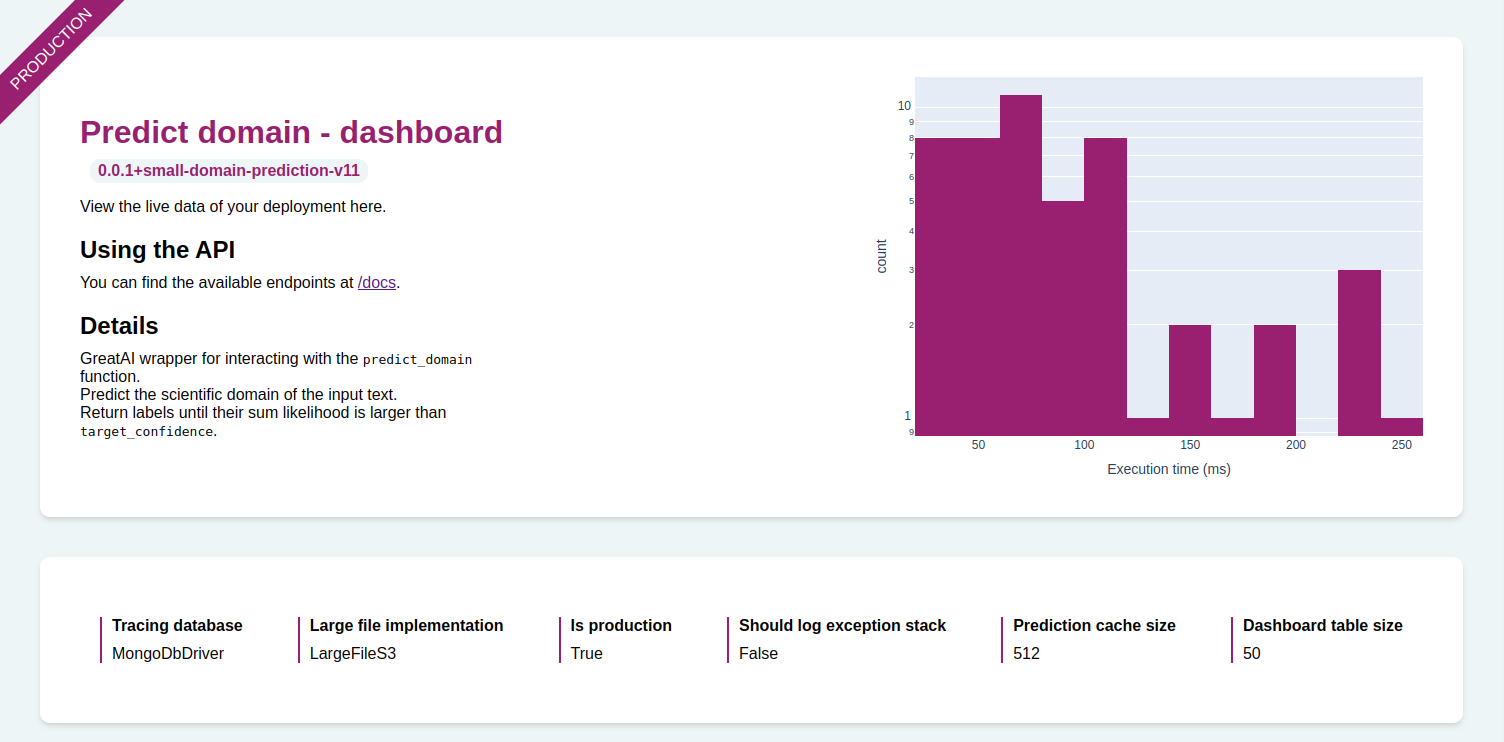
\includegraphics[width=0.9\linewidth]{figures/greatai-header.png}
    \caption{}
    \label{fig:greatai-header}
\end{figure}

\begin{figure}
    \centering
    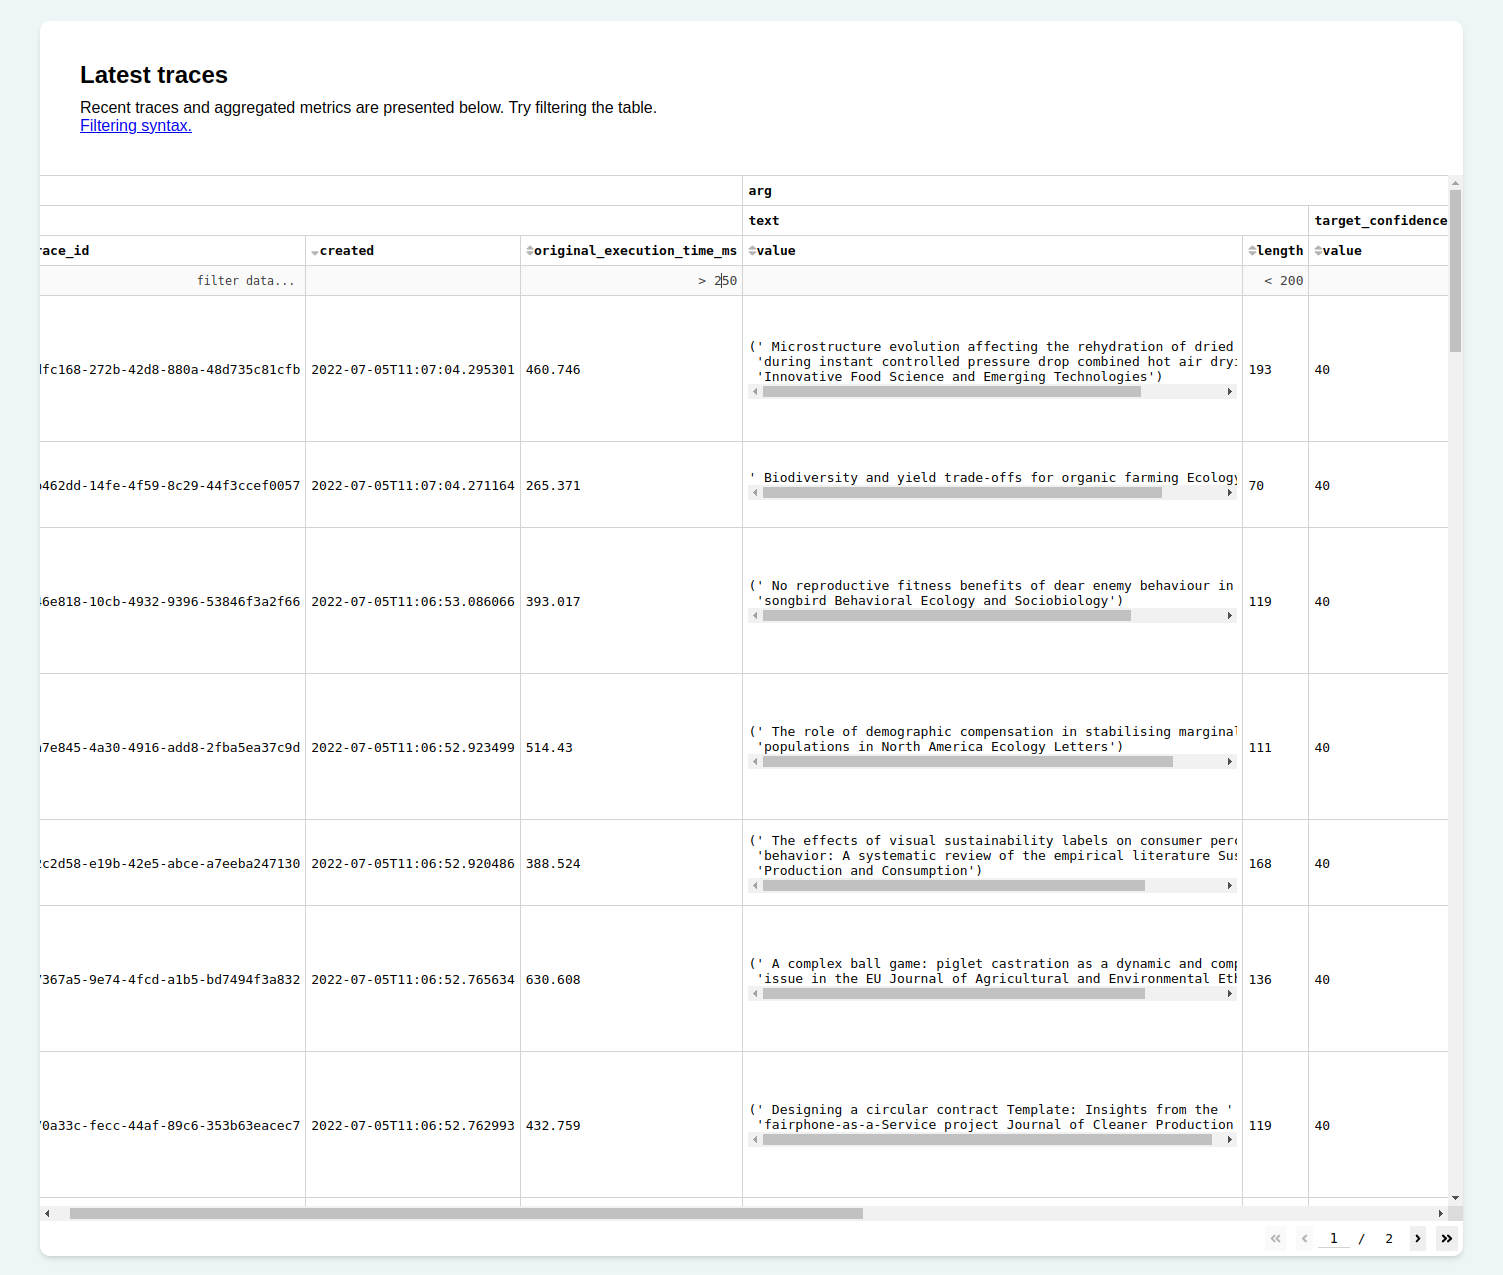
\includegraphics[width=1\textwidth]{figures/greatai-table.png}
    \caption{}
    \label{fig:greatai-table}
\end{figure}

\begin{figure}
    \centering
    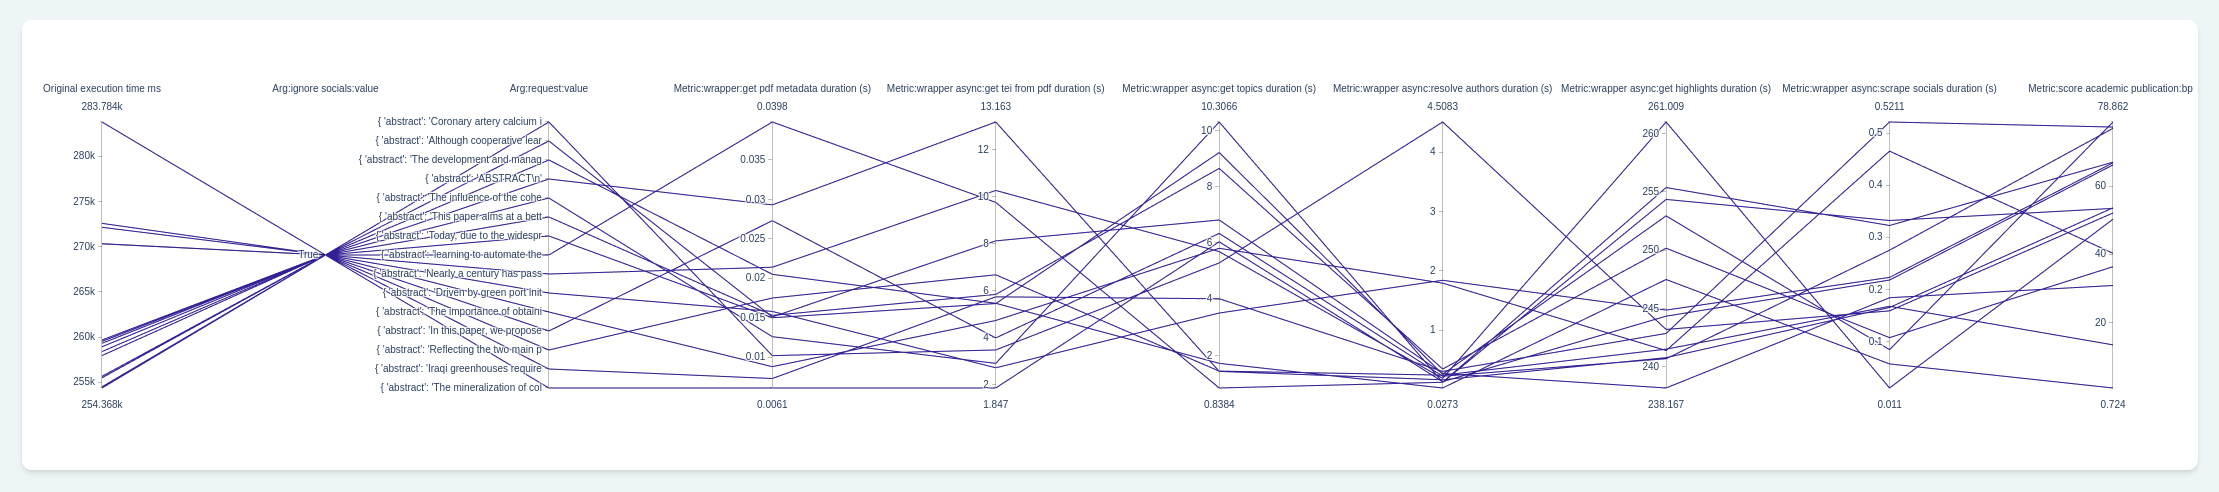
\includegraphics[width=1\textwidth]{figures/greatai-parallel.png}
    \caption{}
    \label{fig:greatai-parallel}
\end{figure}


\begin{table}
\centering
\caption{A subset of the AI lifecycle \href{https://se-ml.github.io/practices/}{best practices identified by Serban et al.} \cite{serban2020adoption,serban2021practices} and the level of support GreatAI provides for them. \textit{Full} requires no action from the user, \textit{Partial} requires at least some involvement, while \textit{Slight} provides some useful features but the client is still expected to make a significant effort.}
\label{table:best-practices}
\begin{tabular}{p{7cm}@{\hskip 0.5cm}c@{\hskip 0.5cm}c}
\hline
\textbf{Best practice} & \textbf{Implementation} & \textbf{Level of support} \\\hline

Use Sanity Checks for All External Data Sources  & \texttt{great\_ai.parameter} & Partial \\\hline
Check that Input Data is Complete, Balanced and Well Distributed  & Type-checked input & Slight \\\hline
Write Reusable Scripts for Data Cleaning and Merging & \texttt{great\_ai.utilities} & Partial \\\hline
Make Data Sets Available on Shared Infrastructure (private or public) & \texttt{great\_ai.large\_file} & Full \\\hline

Test all Feature Extraction Code & \texttt{great\_ai.utilities} & Partial \\\hline
Employ Interpretable Models When Possible & \texttt{great\_ai} & Slight \\\hline
Enable Parallel Training Experiments & \texttt{great\_ai.parallel\_map} & Partial \\\hline
Continuously Measure Model Quality and Performance & \texttt{great\_ai} & Full \\\hline
Use Versioning for Data, Model, Configurations and Training Scripts & \texttt{great\_ai.large\_file} & Full \\\hline

Run Automated Regression Tests & \texttt{great\_ai} & Full \\\hline
Use Continuous Integration & Docker Images \& scripts & Partial \\\hline
Use Static Analysis to Check Code Quality & Typed API & Partial \\\hline
Assure Application Security & GreatAI is audited & Partial \\\hline

Automate Model Deployment & Docker Images \& scripts & Partial \\\hline
TODO: Enable Shadow Deployment & GreatAI & Full \\\hline
Continuously Monitor the Behaviour of Deployed Models & \texttt{great\_ai} & Full \\\hline
Enable Automatic Roll Backs for Production Models &  Docker Images & Partial \\\hline
Log Production Predictions with the Model's Version and Input Data & GreatAI & Full \\\hline

Explain Results and Decisions to Users & GreatAI & Slight \\\hline
\end{tabular}
\end{table}


Table \ref{table:best-practices} summarises the implemented best practices.
